\section{Multilateration Lokalisierung}
\label{sec:gradient_localization}

Der Algorithmus startet beim Setup der Simulation mit der Bestimmung der Hop Counts von allen Personen zu allen Ausgängen. Der \emph{Hop Count} repräsentiert im Netzwerk die Anzahl der Sprünge, die benötigt wird, um einen Knoten zu erreichen. Sei beispielsweise ein Notausgang mit einer Person verbunden, so hat sie einen Hop Count von 1 vom Notausgang aus. Ist diese Person mit einer anderen Person verbunden, die wiederum \emph{nicht} mit dem Notausgang verbunden ist, so hat sie einen Hop Count von 2.

\paragraph{Theorie} 

Nachdem die geschätzten Distanzen zu den Orientierungspunkten (Notausgängen) zu jeder Person berechnet sind, ist es möglich, eine Abschätzung der Position dieser Person zu machen. Dafür benötigt man mindestens 3 Punkte, es werden jedoch wesentlich mehr Punkte benötigt, um eine bessere Approximation zu der echten Position zu erreichen (vergleiche \cite{Jonathan.2004} ab Seite 217, Kapitel Analysis). 

\begin{equation} \label{eq:dist}
d_{ij} = \sqrt{(x_i - x_j)^2 + (y_i - y_j)^2}
\end{equation}

In der Formel \ref{eq:dist} bestimmen wir die Formel, die die Distanz zwischen einem Orientierungspunkt j und einem beliebigen Punkt i beschreibt. Das benutzen wir, um die tatsächliche Distanz zu der Person mit der Distanz zum geschätzten Punkt zu vergleichen.

\begin{equation} \label{eq:error}
E_j = \sum_{i=1}^{n} (d_{ji} - \hat d_{ji})^2
\end{equation}

In der Formel \ref{eq:error} bestimmt die Summe des quadrierten Fehler, d.h. die Fehleinschätzung unserer geschätzten Distanz zu der tatsächlichen Distanz. Dabei ist \( d \) die tatsächliche Position und \( \hat d \) die geschätzte Position. Nun ist also \( d \) die unbekannte und wir wollen diesen Fehler minimieren.

\begin{equation} \label{eq:abl}
 \frac{\partial E_j}{\partial x_i} = \sum_{i=1}^{n}(x_j - x_i) \left( 1-\frac{d_{ji}}{\hat d_{ji}} \right) \textrm{ and }  \frac{\partial E_j}{\partial y_i} = \sum_{i=1}^{n}(y_j - y_i) \left( 1-\frac{d_{ji}}{\hat d_{ji}} \right)
\end{equation}

Um den Fehler zu minimieren bilden wir die partiellen Ableitungen in \ref{eq:abl} und versuchen so, nach Methoden der Analysis, das Minimum zu bestimmen. Wir starten also mit einer geschätzten Position \( \hat d \) und verschieben langsam die Punkte um \( \alpha \) und minimieren damit den Fehler.

\paragraph{Implementierung} 

\begin{figure}[h!]
\centering
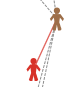
\includegraphics{algorithmik/visu}
\caption{Visualisierung der geschätzten Positionen}
 \label{visu}
\end{figure}

In der Implementierung wählen wir als Punkt \( \hat d \) den Ausgang, der dem Charakter laut hop count am nächsten steht, da jede Person die Position aller Notausgänge im Netzwerk kennt. Bei der Implementierung orientiert sich der Algorithmus an den Referenzcode der zur Verfügung gestellt wurde. Nachdem der Hop Count beim Setup für jede Person bestimmt wurde, kann der Algorithmus für jede Person ausgeführt werden. Wieviele Iterationen vorgenommen werden, ist ein einstellbarer Parameter. Nachdem eine Position für eine Person geschätzt wurde, wird sie als rote Person in die Simulationsumgebung integriert und mit der richtigen Person mit einem roten Link verbunden, wie auf der Abbildung \ref{visu} zu sehen ist.




